\section{机会判别与人工复核}

\subsection{全量自动判别}

模型对 2,561 条清洗记录执行结构化判别，覆盖率为 100\%。原模型标记 269 条候选机会、2,292 条非机会。模型服务返回结构化结果，程序检查 record\_id 集合、标签合法性、机会逻辑和正文证据；全文中无法定位的证据会使批次重试。原模型累计使用 2,872,796 个输入 token 和 588,074 个输出 token，服务单价未配置，成本未知。

原模型的置信度是模型自评值，未进行概率校准。因而本文只把它用于筛选和流程计算，不将其写成已验证概率。

\subsection{分层复核队列}

复核队列包含全部 269 条模型候选机会，以及 240 条模型非机会样本。负例按来源网站和内容类型轮转，并在各层内优先选择模型置信度较低的记录。这样的设计适合查找模型边界和难例，但不是简单随机抽样，不能用来无偏估算 2,292 条模型非机会记录的整体漏判率。

图~\ref{fig:review-composition} 按来源和正文类型展示 509 条人工复核记录及其确认标签。复核样本中 Hacker News 占 282 条，GitHub 占 99 条；人工确认机会主要出现在 Hacker News 和量子位。该结构来自对原模型正例的全量纳入及定向负例抽样，不能解释为来源间机会率差异。

\begin{figure}[H]
  \centering
  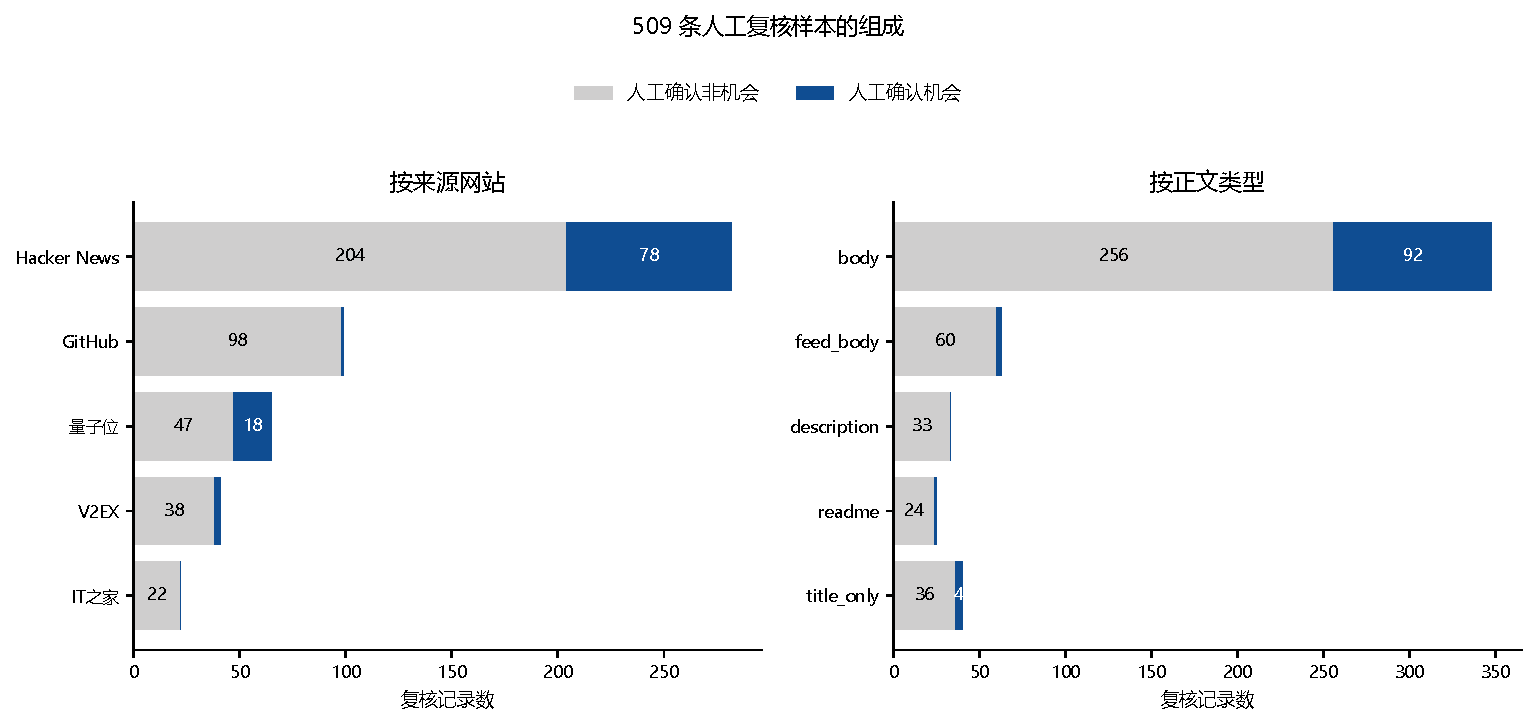
\includegraphics[width=0.98\textwidth]{../figures/fig09_review_sample_composition.pdf}
  \caption{509 条人工复核样本按来源网站和正文类型分组。颜色区分人工确认机会与人工确认非机会；样本构成为分层抽样结果。}
  \label{fig:review-composition}
\end{figure}

\subsection{可见标签、盲复核与 AI 裁定}

第一轮辅助复核同时提供正文和原模型字段；第二轮盲复核只提供记录文本和来源元数据。两轮都由同一模型完成，分别给出 141 条和 109 条机会判断；两轮判断一致 419 条，占 82.32\%。原模型与可见标签复核一致 379 条，与盲复核一致 337 条；三者同时一致 313 条，占 61.49\%。另有 328 条记录因判断分歧、边界标记或功能行业分类不一致进入再次裁定，这个集合不能等同于 328 条二分类分歧。

\begin{table}[H]
  \centering
  \caption{模型标签之间的一致记录数}
  \label{tab:review-agreement}
  \begin{tabular}{lrr}
    \toprule
    对照结果 & 一致记录数 & 占复核队列比例 \\
    \midrule
    可见标签辅助复核与盲复核 & 419 & 82.32\% \\
    原模型与可见标签辅助复核 & 379 & 74.46\% \\
    原模型与盲复核 & 337 & 66.21\% \\
    原模型、可见标签及盲复核三方一致 & 313 & 61.49\% \\
    \bottomrule
  \end{tabular}
\end{table}

表~\ref{tab:review-agreement} 中的比例衡量同一组模型输出之间的一致程度，不是准确率。由于所有判断均来自同一模型，输入提示及先前标签可能造成相关误差。

对这 328 条记录再次调用模型辅助裁定，并将 181 条稳定共识保留，形成覆盖 509 条队列的人工复核结果。其中 100 条为人工确认机会，占队列的 19.65\%；169 条相对原模型发生标签变化，占 33.20\%；160 条标记为边界情况。复核结果保留原模型标签、辅助复核结果和来源证据；用户随后阅读全部 509 条材料并确认对应分类，人工复核字段保存确认类别，备注为空。图~\ref{fig:labelshift} 展示人工确认标签相对原模型的变化。

\begin{figure}[H]
  \centering
  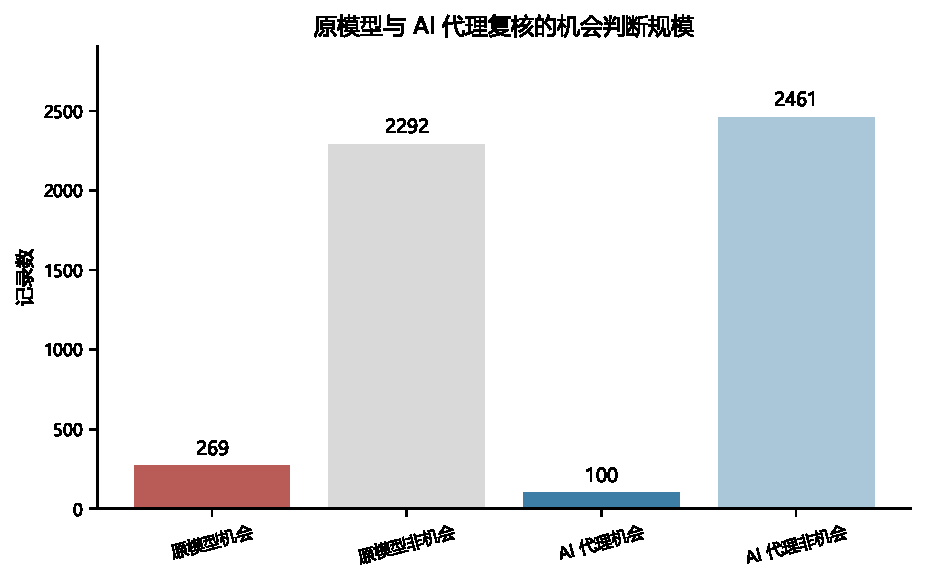
\includegraphics[width=0.82\textwidth]{../figures/fig04_label_shift.pdf}
  \caption{原模型与人工确认结果中的机会判断规模。全量结果包含 509 条人工复核标签及 2,052 条未复核原模型标签，因此该图不表示全量分类准确率。}
  \label{fig:labelshift}
\end{figure}

\subsection{面向人工复核标签的文本分类比较}

为比较小样本条件下不同文本模型对人工复核标签的复现能力，本文纳入 509 条记录，其中 100 条机会、409 条非机会。输入文本由标题与正文拼接，并截取至 12,000 个字符。模型包括字符 2--5 gram TF-IDF 逻辑回归和 ComplementNB，以及多语言 E5 冻结向量上的逻辑回归、RBF-SVM 和 MLP。TF-IDF 在每个训练折拟合，最低词频为 2，最多保留 50,000 个特征，并采用子线性词频缩放与 0.98 的文档频率上限。逻辑回归使用 $C=1$；ComplementNB 使用 $\alpha=1$ 和归一化；RBF-SVM 使用 $C=1$、尺度自适应核参数及三折 sigmoid 校准。

E5 使用固定 revision 的 multilingual-e5-small，将输入截断至 512 个 token，输出 384 维向量，经注意力掩码均值池化和 L2 归一化。每个外层训练折单独拟合标准化器。MLP 隐藏单元候选为 8 或 16，正则化系数为 0.1 或 1.0；三折内层验证按平均精确率选参，学习率为 0.001，最多迭代 1,000 次，并采用平衡样本权重。所有模型使用外层五折交叉验证并重复两次；外层随机种子为 20261119。类别权重或平衡样本权重仅应用于训练数据。阈值 0.5 下报告 Macro-F1 与平衡准确率，同时报告平均精确率、ROC-AUC 及外层折间标准差。该标准差描述折间变异，不是置信区间。人工确认机会占 19.65\%，因此主要关注对类别不平衡较稳健的平均精确率。

表~\ref{tab:proxy-classifiers} 给出 10 个外层折的均值与标准差。字符 TF-IDF 逻辑回归的平均精确率最高，为 0.488；在冻结 E5 表示上，RBF-SVM 与 MLP 均高于 E5 逻辑回归。RBF-SVM 的平衡准确率为 0.720，是五种方法中的最高值。MLP 所有内外层拟合均收敛。不同指标的模型排序并不相同，当前样本不足以支持某一种方法普遍更优的结论。

\begin{table}[H]
  \centering
  \small
  \caption{人工复核标签上的嵌套交叉验证比较}
  \label{tab:proxy-classifiers}
  \begin{tabular}{lrrr}
    \toprule
    方法 & 平均精确率 & Macro-F1 & 平衡准确率 \\
    \midrule
    字符 TF-IDF + 逻辑回归 & $0.488\pm0.077$ & $0.661\pm0.036$ & $0.679\pm0.044$ \\
    字符 TF-IDF + ComplementNB & $0.459\pm0.089$ & $0.464\pm0.056$ & $0.648\pm0.061$ \\
    冻结 E5 + 逻辑回归 & $0.367\pm0.056$ & $0.614\pm0.056$ & $0.632\pm0.059$ \\
    冻结 E5 + RBF-SVM & $0.445\pm0.055$ & $0.660\pm0.049$ & $0.720\pm0.054$ \\
    冻结 E5 + 内层选择 MLP & $0.441\pm0.064$ & $0.643\pm0.034$ & $0.644\pm0.037$ \\
    \bottomrule
  \end{tabular}
\end{table}

图~\ref{fig:proxy-comparison} 汇总三种主要方法的折间指标，图~\ref{fig:classifier-family} 展示五种模型族的平均精确率与 ROC-AUC。图~\ref{fig:proxy-oof} 展示字符 TF-IDF、冻结 E5 逻辑回归和 MLP 的折外平均精确率—召回率曲线与阈值 0.5 混淆矩阵。这三种方法分别在 51、49 和 44 条记录上正确复现人工确认机会；该数量只比较复核样本，不代表全批次机会数量。

\begin{figure}[H]
  \centering
  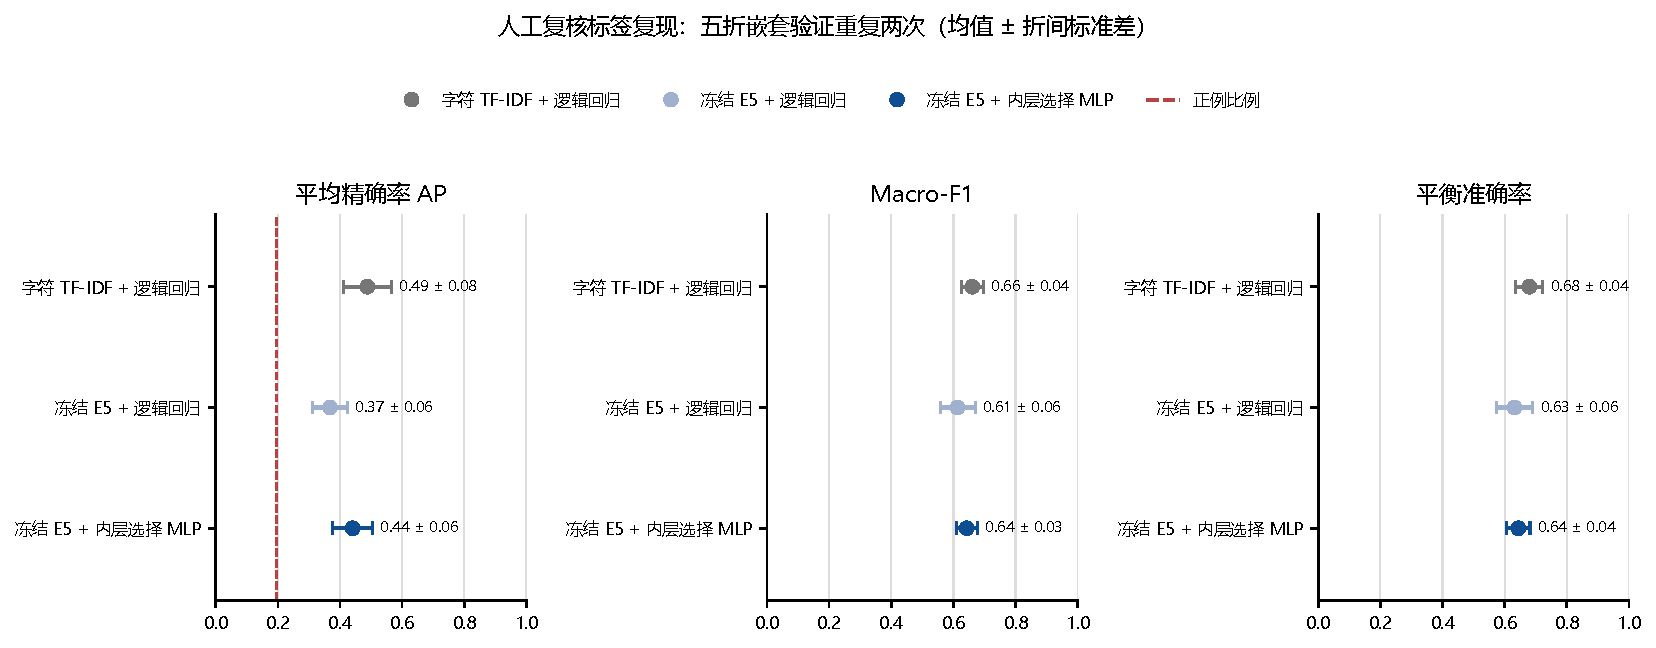
\includegraphics[width=0.98\textwidth]{../figures/fig10_proxy_classifier_comparison.pdf}
  \caption{509 条人工复核记录的重复五折外层交叉验证结果。点和误差线表示 10 个外层折的均值与标准差；红色虚线为复核样本机会比例。误差线不是置信区间。}
  \label{fig:proxy-comparison}
\end{figure}

\begin{figure}[H]
  \centering
  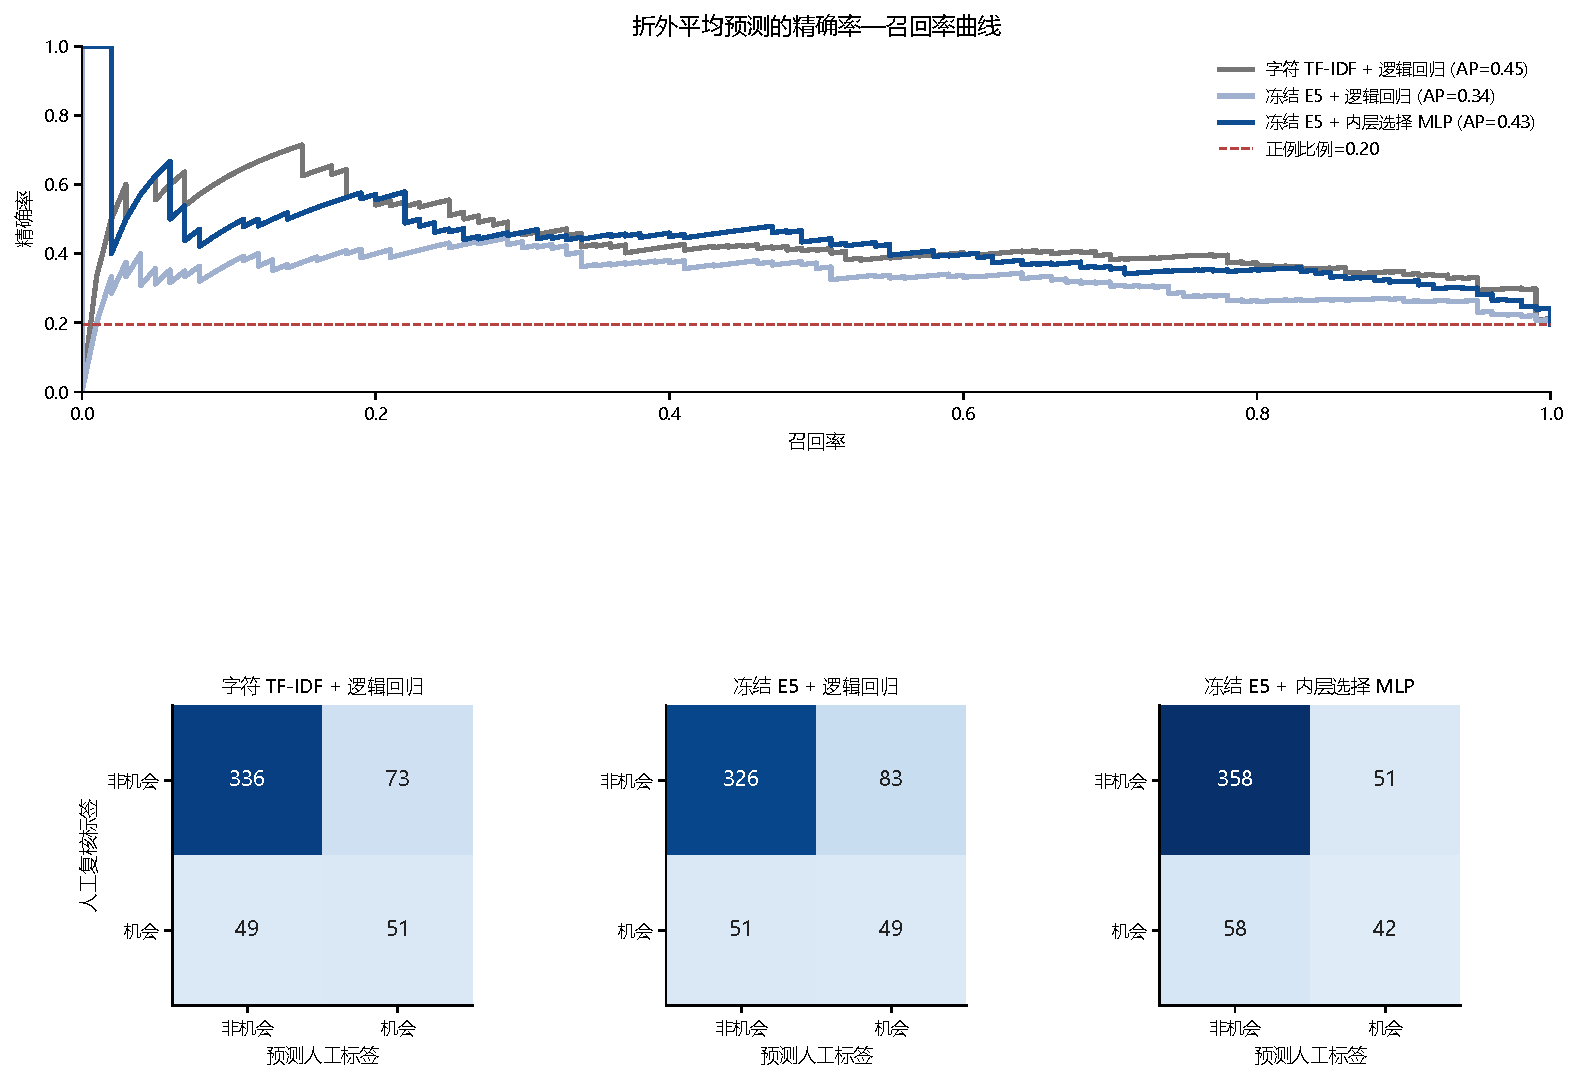
\includegraphics[width=0.98\textwidth]{../figures/fig11_proxy_classifier_oof.pdf}
  \caption{外层折外平均概率的精确率—召回率曲线及混淆矩阵。图中参照标签来自人工复核；结果不外推到未复核记录。}
  \label{fig:proxy-oof}
\end{figure}

\begin{figure}[H]
  \centering
  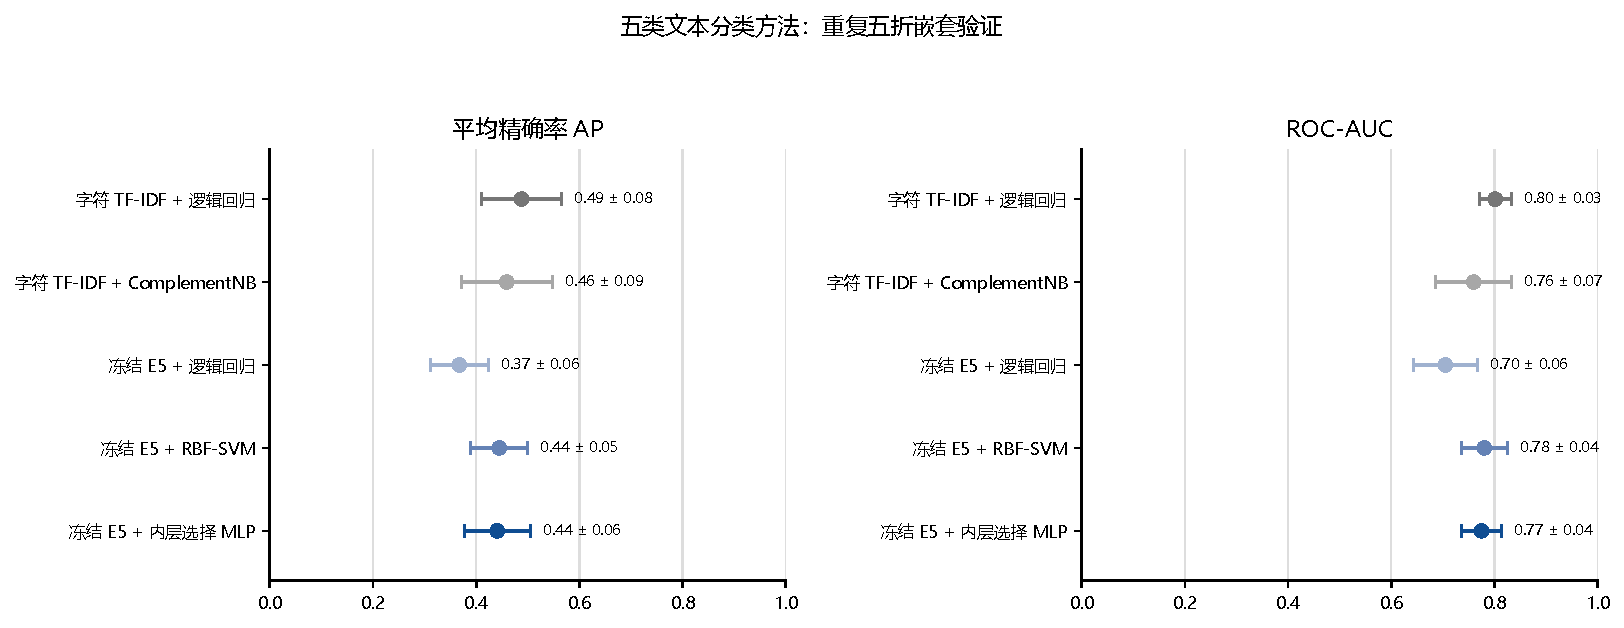
\includegraphics[width=0.98\textwidth]{../figures/fig16_classifier_family.pdf}
  \caption{五种模型族在人工复核标签上的重复嵌套验证结果。误差线为外层折间标准差；E5-RBF-SVM 经外层训练集内的 sigmoid 校准。}
  \label{fig:classifier-family}
\end{figure}

图~\ref{fig:embedding-pca} 将复核样本的 E5 向量压缩至两个主成分。两类标签在二维投影中明显交叠，且该投影仅解释向量总方差的 22.2\%；它用于观察表示空间结构，不作为分类边界或簇质量的检验。

为考察跨来源迁移，另进行留一来源验证：每次将一个网站的复核记录整体留作测试，其余四个来源用于训练，MLP 参数在训练来源内单独选择。五个来源的机会正例数量分别为 Hacker News 78 条、GitHub 1 条、量子位 18 条、V2EX 3 条和 IT 之家 0 条；因此 IT 之家留出时平均精确率与 ROC-AUC 不可估，其余来源的指标也受正例数稀少限制。图~\ref{fig:source-holdout} 报告三个主要模型的来源留出平均精确率，展示跨来源变化，不把这些小组样本分数合并为单一泛化估计。

\begin{figure}[H]
  \centering
  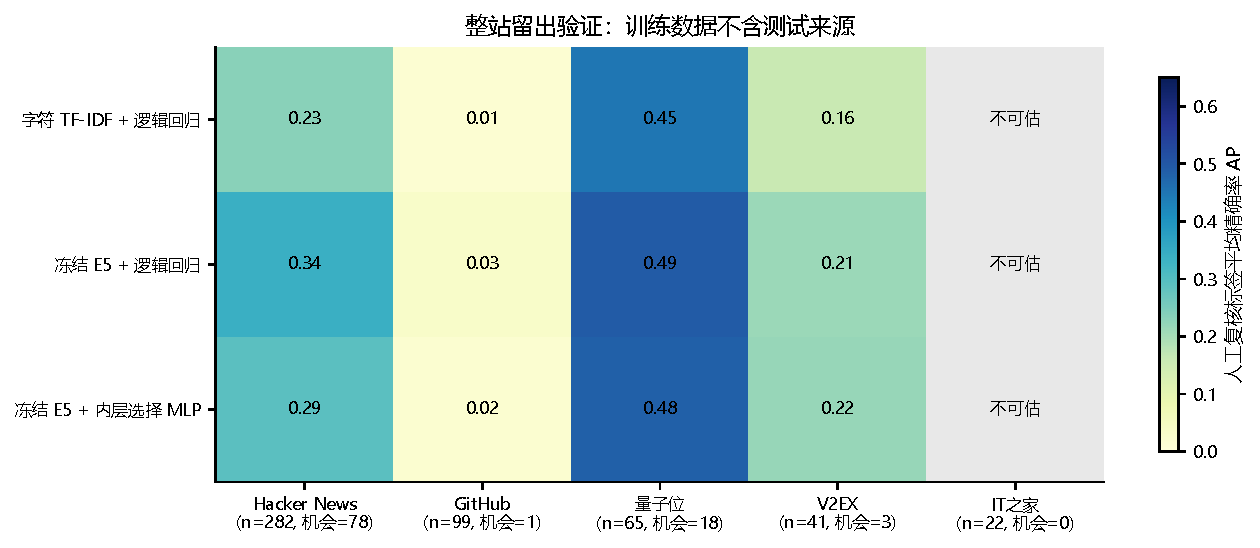
\includegraphics[width=0.98\textwidth]{../figures/fig17_source_holdout.pdf}
  \caption{留一来源验证的人工复核标签平均精确率。横轴同时列出留出来源的样本数和人工确认机会数；无正例来源不计算平均精确率。各来源正例数偏少，图中分数用于显示迁移差异。}
  \label{fig:source-holdout}
\end{figure}

\begin{figure}[H]
  \centering
  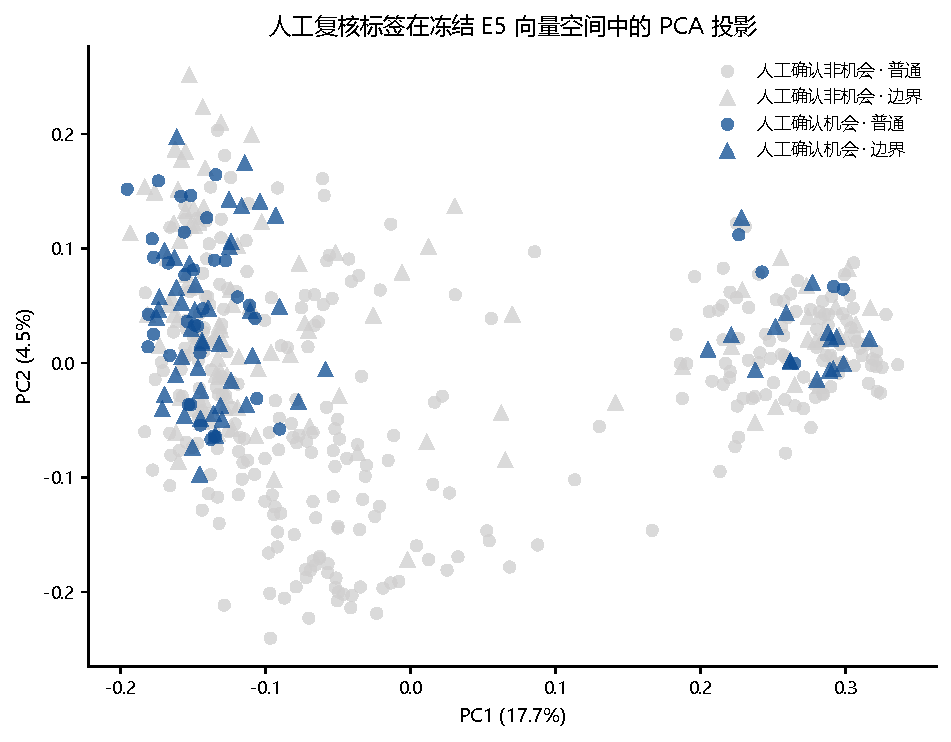
\includegraphics[width=0.76\textwidth]{../figures/fig12_embedding_pca.pdf}
  \caption{人工复核样本在冻结 E5 向量空间的 PCA 投影。符号区分被标记为边界的记录，颜色表示人工确认标签。}
  \label{fig:embedding-pca}
\end{figure}

该比较使用 509 条人工确认标签。人工字段记录确认类别，备注为空；模型辅助复核过程保留在 AI 使用记录中。复核队列的负例经过定向抽样，未进入队列的 2,052 条记录仍沿用原模型标签。因此交叉验证只描述人工复核样本，不能外推到全量记录。
